\documentclass[12pt]{report}
\usepackage[T1]{fontenc}
\usepackage[utf8]{inputenc}
\usepackage{graphicx}
\usepackage{hyperref}
\usepackage[explicit]{titlesec}
\usepackage{color, varwidth}
\usepackage[margin=0.75in]{geometry}
\usepackage{xhfill}

\graphicspath{{./images/}}

%----------------------------------------------------------------------------------------
%	ROMAN NUMERALS
%----------------------------------------------------------------------------------------

\usepackage{outlines}
\usepackage{enumitem}
\setenumerate[1]{label=\Roman*.}
\setenumerate[2]{label=\bullet}
\setenumerate[3]{label=\roman*.}
\setenumerate[4]{label=\alph*.}


%----------------------------------------------------------------------------------------
%	SECTION HEADER STYLES
%----------------------------------------------------------------------------------------
\setlength{\headheight}{15pt}

\definecolor{darkblue}{RGB}{0,101,135}
\definecolor{ourblue}{RGB}{0,138,184}

\newcommand{\hsp}{\hspace{20pt}}
\titleformat{\chapter}[hang]{\huge\bfseries}{\thechapter\hsp\textcolor{ourblue}{|}\hsp}{0pt}{#1\Huge\bfseries}

\newcommand\Centered{%
\titleformat{\section}[hang]
  {\normalfont\large\filcenter}{}{0em}
  {\xrfill[0.3ex]{1.0pt}[ourblue]~\begin{varwidth}{.75\linewidth}\centering{\color{darkblue}##1}\end{varwidth}~\xrfill[0.3ex]{1.0pt}[ourblue]}
}

\newcommand\textline[4][t]{%
  \par\smallskip\noindent\parbox[#1]{.333\textwidth}{\raggedright#2}%
  \parbox[c]{.333\textwidth}{\centering#3}%
  \parbox[c]{.333\textwidth}{\raggedleft#4}\par\smallskip%
  \vspace{.5\baselineskip}
}

\titlespacing{\chapter}{12pt plus 4pt minus 2pt}{\parskip}{7pt}


\renewcommand\sectionmark[1]{\markboth{#1}{}}

%----------------------------------------------------------------------------------------

\begin{document}

\begin{titlepage}
\begin{center}

\newcommand{\HRule}{\rule{\linewidth}{0.5mm}}


\includegraphics[width=0.25\textwidth]{purdue_seal.png}~\\[1cm]

\vspace{10mm}



\includegraphics[width=0.6\textwidth]{logo.png}~\\[1cm]

% Title
\HRule \\[0.4cm]
{ \huge \bfseries Design Document \\[0.4cm] }

\HRule \\[1.5cm]

% Author and supervisor
\noindent
\begin{minipage}{0.4\textwidth}
\begin{flushleft} \large
Abhijeet \textsc{Chakrabarti}\\
Ammar \textsc{Askar}\\
Brian \textsc{Quinn}\\
Eric \textsc{Lee}
\end{flushleft}
\end{minipage}%
\begin{minipage}{0.4\textwidth}
\begin{flushright} \large
\textsc{Team }\#29
\end{flushright}
\end{minipage}

\vfill

% Bottom of the page
{\large \today}

\end{center}
\end{titlepage}

\tableofcontents

\pagebreak

\chapter{Purpose}
The music streaming industry has been surging to new heights, growing 76\% in the U.S. in 2016. Synchronizo aims to bring people together to enjoy listening to music in real-time. You can be anywhere in the world and still, listen to music with your friends who are miles away. This will be different from current music streaming services where you can share songs passively but not listen to them with people as if they were in the same room as you.
Applications such as Spotify allow people to stream music alone or from playlists made by other people but does not support concurrent listening. Services such as Youtube synchronization websites allow for simultaneous music listening but in an unorganized and loose fashion.

\Centered{
    \section{Functional Requirements}
}

\begin{enumerate}
   \item \textbf{Music Streaming and Uploads}
       \begin{itemize}
           \item Listeners will be able to upload music files to the music player from their own computer.
       \end{itemize}
    \item \textbf{Social Networking}
        \begin{itemize}
            \item Users will be able to create their own account.
            \item Users will be able to follow and unfollow other users.
            \item Users will be able to set privacy settings on their account.
            \item Users will be able to direct message other users.
            \item Users will be able to block other users.
            \item Users will be able to invite other users to join their listening party.
            \item Users will be able to party chat with other users in the same listening party.
            \item Users will be able to personalize their profile with pictures, bio, and their favorite music.       
        \end{itemize}
    \item\textbf{Music Playback}
        \begin{itemize}
            \item Listeners will able to play, pause, skip and replay the current track.
            \item Listeners will be able to see album cover art and artist info on the track that is currently playing.
        \end{itemize}
    \item\textbf{Managing Accounts}
        \begin{itemize}
            \item Administrators will have the ability to add user accounts.
            \item Administrators will be able to ban or delete user accounts as necessary.
        \end{itemize}
\end{enumerate}

\Centered{
    \chapter{Design Outline}
}
\section{High Level Overview}
Synchronizo's model is based on a Client-Server architecture. The server keeps track of the state of the music room, this ephemeral information includes things like the currently playing track, the time stamp at which it is playing, queued up songs etc. The clients get updates pushed to them when this state changes, for example when another user uploads a new music track or seeks a song. Clients then act upon these updates and re-render the page appropriately.

\begin{center}
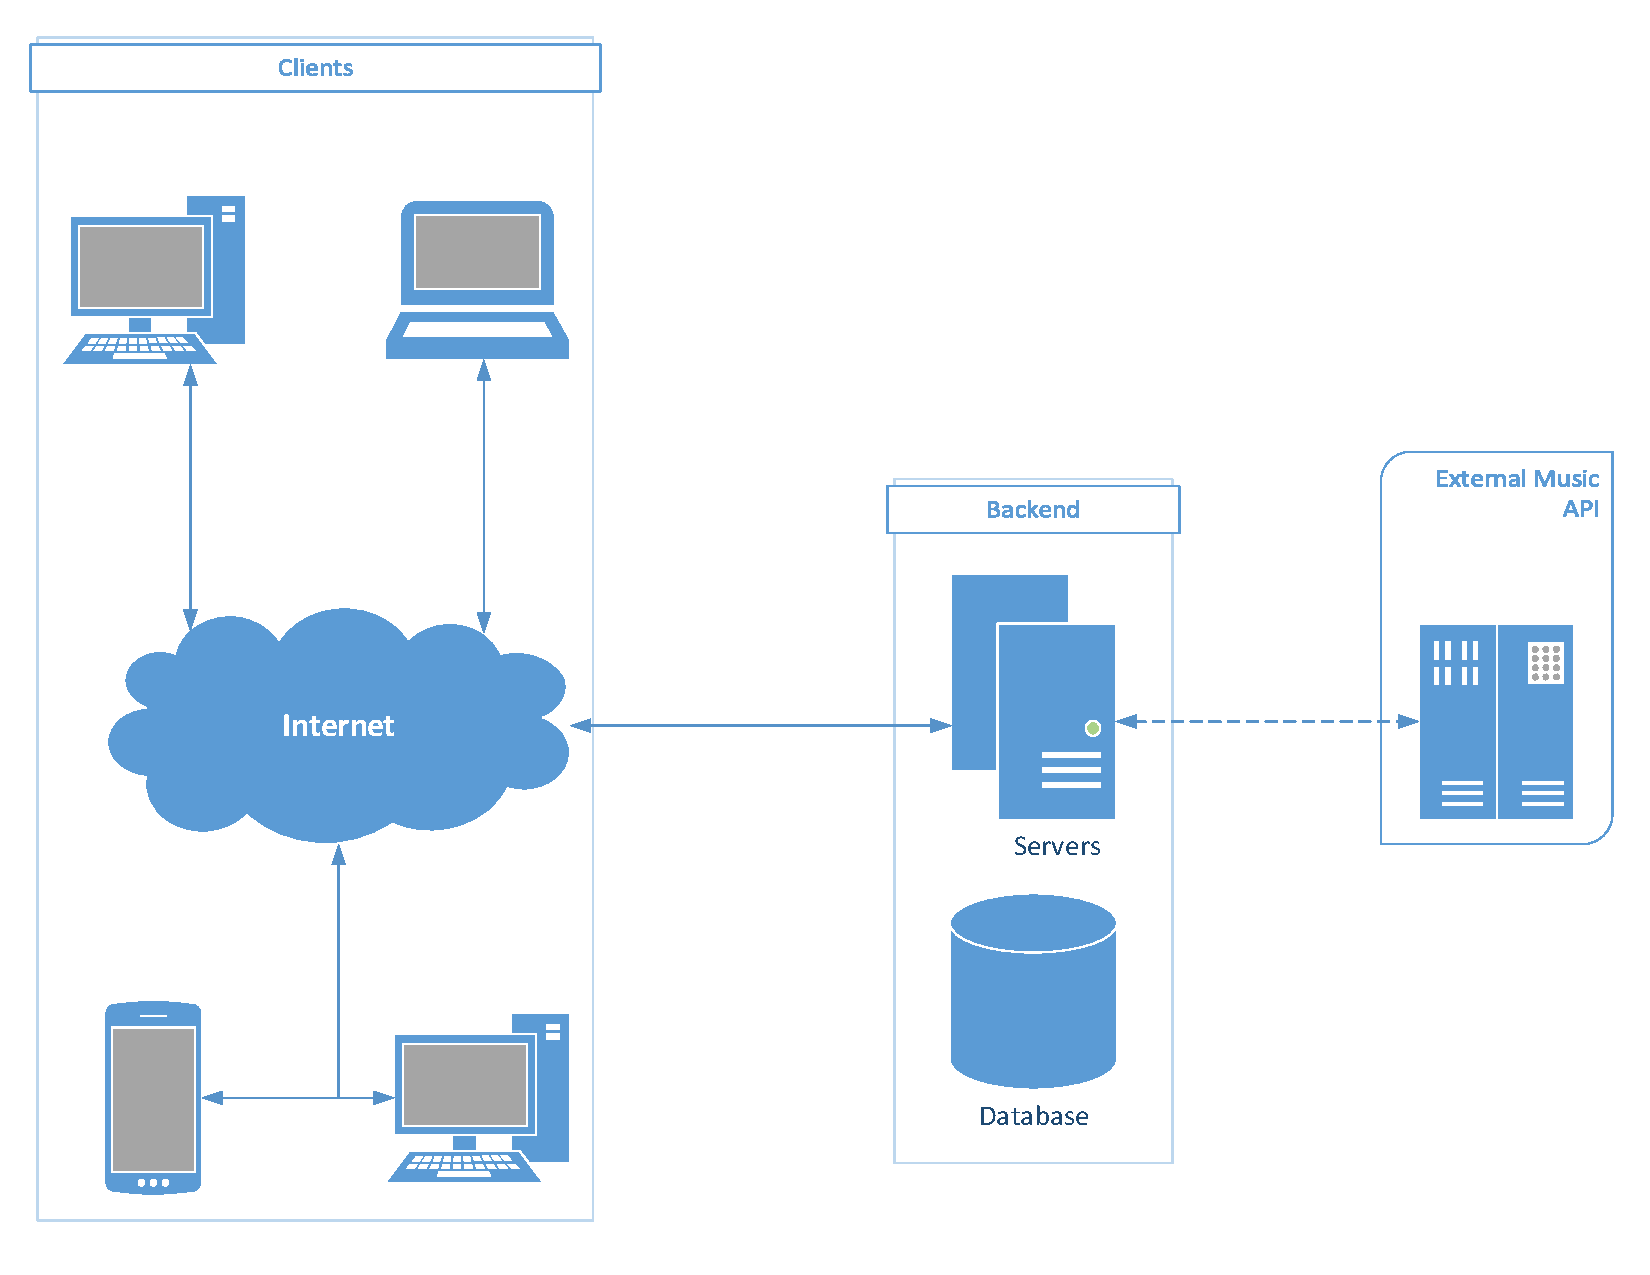
\includegraphics[scale=0.65]{highlevel.pdf}
\end{center}

\begin{enumerate}
    \item Client
    
        Upon opening the Synchronizo web page, the user's web browser establishes a WebSocket/Long Polling connection to the backend server to establish a communication line.
        
        The client listens for data on this connection, and has updates pushed to it by the client. Upon receiving an update, it renders it appropriately. For example, a new song being added would cause it to render a new box displaying the newly added track. A user leaving the room could be marked with a notification badge etc.
    
    \item Server
    
        The server serves static html/css files in addition to listening for connections from clients. Upon a connection being established, the server adds it to the pool of currently connected users. When updates need to be pushed, the server iterates through the pool of connected clients, filters to the ones in appropriate rooms and then sends them the update data.
        
        This data is considered temporary/ephemeral because the state of a music room only needs to be preserved while a server is running, there is no point in keeping this in a permanent such as a database because this will only negatively affect performance and add needless complexity.
        
    \item Database
    
        The database is in charge of storing all the non-ephemeral data such as user account information and long term listening history. The server will query the database for this information when certain actions are taken such as when a user logs in.
        
        More persistent data such as a user's long term's music taste will also be stored here. Eventually, when the social networking aspects of the site are built out, this will also contain information about the user's friends, information about their profile page etc.
    
    \item External Music API
        
        The external music API is a potential source for retrieving audio files so they can be served to the user. The server will be responsible for communicating with this API (likely through their HTTP API). The external music API will also be used to retrieve information such as artist name, album art, year, artist biography for songs that are uploaded by users since often enough these audio files lack full and proper metadata.
    
\end{enumerate}
\chapter{Design Issues}

\section{What type of architecture should we use?}
\begin{itemize}
    \item{Monolithic Architecture}
    \item{Micro-Services Architecture}
    \item\textbf{Client-Server Architecture}
\end{itemize}
As Synchronizo is a web-application, the immediately obvious choice for implementation architecture is a Client-Server model, especially since HTTP itself implicitly requires servers and clients. To elaborate on this a little, the clients will be the users on their browsers while the server, running a node.js web-app, will keep track of the state of music rooms and push updates to clients when changes occur. In addition to this ephemeral data, it will also keep permanent data in a database.

On the backend side of things, we could potentially implement the backend as a Monolith, or with Micro-Services. We've chosen to go with an extensible monolith since we believe this application will be simple enough to justify not having the added complexity of inter-service communication.


\section{What will be the source of our music?}
\begin{itemize}
    \item{Spotify}
    \item{Soundcloud}
    \item\textbf{Users Upload Their Own Music}
\end{itemize}
The music that our listeners have access to will ultimately be dependent on users uploading their own files. After careful consideration of the terms and conditions of the APIs' of both Spotify and Soundcloud, we decided that a possible conflict of interest could arise if we tried to implement their APIs' in our service. 

\section{What front end framework should we use?}
\begin{itemize}
    \item{Foundation}
    \item{Pure}
    \item{Our own HTML+CSS from scratch}
    \item\textbf{Bootstrap} 
\end{itemize}
To create a decent looking front-end from scratch would take a significant amount of time, which is why frameworks like Bootstrap/Foundation/Pure exist. They allow for rapid prototyping and creation of beautiful looking interfaces with significantly reduced time. Due to the authors being experienced with Bootstrap, we went with this option.

\section{What back end language should we use?}
\begin{itemize}
    \item{PHP}
    \item{Python}
    \item{Java}
    \item\textbf{node.js} 
\end{itemize}
When it comes to deciding the language for the back-end server, there are a couple of very solid options that are generally used for web development. Our focus was finding a language that allowed for very simple real-time communication between the browser and the server. PHP is mostly designed to render static pages, or pages with slight dynamic content and not handle active communications so it was instantly off the table. Python has some decent frameworks for real time web-apps but they are very immature and buggy. 

Java has some very mature frameworks, however the verbosity of Java and its frameworks was an instant turn off. In contrast, node.js allows for quick prototyping, and has been tested and proven to be used for exactly these kind of applications. It also has a great deal of supporting libraries specifically tied for web development.


\section{How will the browser and server communicate?}
\begin{itemize}
    \item{Repeated AJAX requests}
    \item{Long Polling}
    \item{Web Sockets}
    \item\textbf{socket.io}
\end{itemize}
Since Synchronizo will work as a web-application with updates occurring in real time, some form of communication line between the server and browsers needs to be established. A very brute force approach would be something along the lines of having the user refresh the web page every few seconds. However, this is highly crude and extremely unfriendly to the user.

Some possible solutions include having javascript send ajax requests to the server every $t$ seconds asking for the latest state. However, this means that we will be firing off requests very often, potentially using up a lot of bandwidth and having a lag time of a maximum $t$ seconds.

Long Polling aims to fix this by making long lives requests that the server only responds to when something changes, however long polling is problematic since it can potentially clutter up a server's TCP response pool, as outlined by \href{https://tools.ietf.org/html/rfc6202}{\color{blue} RFC 6202}.

WebSockets are a relatively new technology that allow for real time communication between a website and browser, but because of how new they are, only more modern browsers support them. This means that we potentially lose a market share of people with older browsers.

socket.io allows for the best of both worlds, using WebSockets and falling back to Long Polling if the browser does not support WebSockets. Additionally, socket.io has excellent integration with node.js which means a great deal of the work of integrating the communication will be done as part of the library.

\section{What sort of protocol will we expose for the API?}
\begin{itemize}
    \item{Proprietary}
    \item{Messaging}
    \item\textbf{RESTful JSON}
\end{itemize}
A method of communication between the browser and server has been established, but now we need to decide what sort of protocol they'll use. We could go with a proprietary text/binary protocol that we create by ourselves, however this is some very heavy NIHS (Not Invented Here Syndrome). We could go with messaging protocols such as those used by RabbitMQ/General message queuing systems, however we decided to use a RESTful JSON API simply because that is the current standard for web applications and allows for a great deal of interoperability such as being able to be consumed by an Android/iOS/Desktop app in addition to the web-app itself.

\section{What design scheme should we use?}
\begin{itemize}
    \item{Fixed}
    \item{Fluid}
    \item{Adaptive}
    \item\textbf{Responsive}
\end{itemize}
A fixed design schema would mean that our application would be limited to looking good on only one size of screen, which is not really acceptable considering we want it to be usable by anyone with a web browser.

For ensuring a consistent user experience, Responsive design is a better choice as it reacts to the size of a user’s screen, thus, optimizing the browsing experience.

\section{What database should we use?}
\begin{itemize}
    \item{MySQL}
    \item{PostgreSQL}
    \item{MongoDB} 
    \item\textbf{All of the Above}
\end{itemize}
Instead of going with a single fixed database for the back-end, we've decided to use an ORM (Object Relational Mapper) that can support any database of the system administrator's choosing. This adds versatility and will avoid writing code specific to a database implementation. This also means we don't directly have to write SQL/MongoDB Query Documents which means we aren't tied down to anything.

\Centered{
    \chapter{Design Details}
}

\section{Class Overview}

\begin{center}
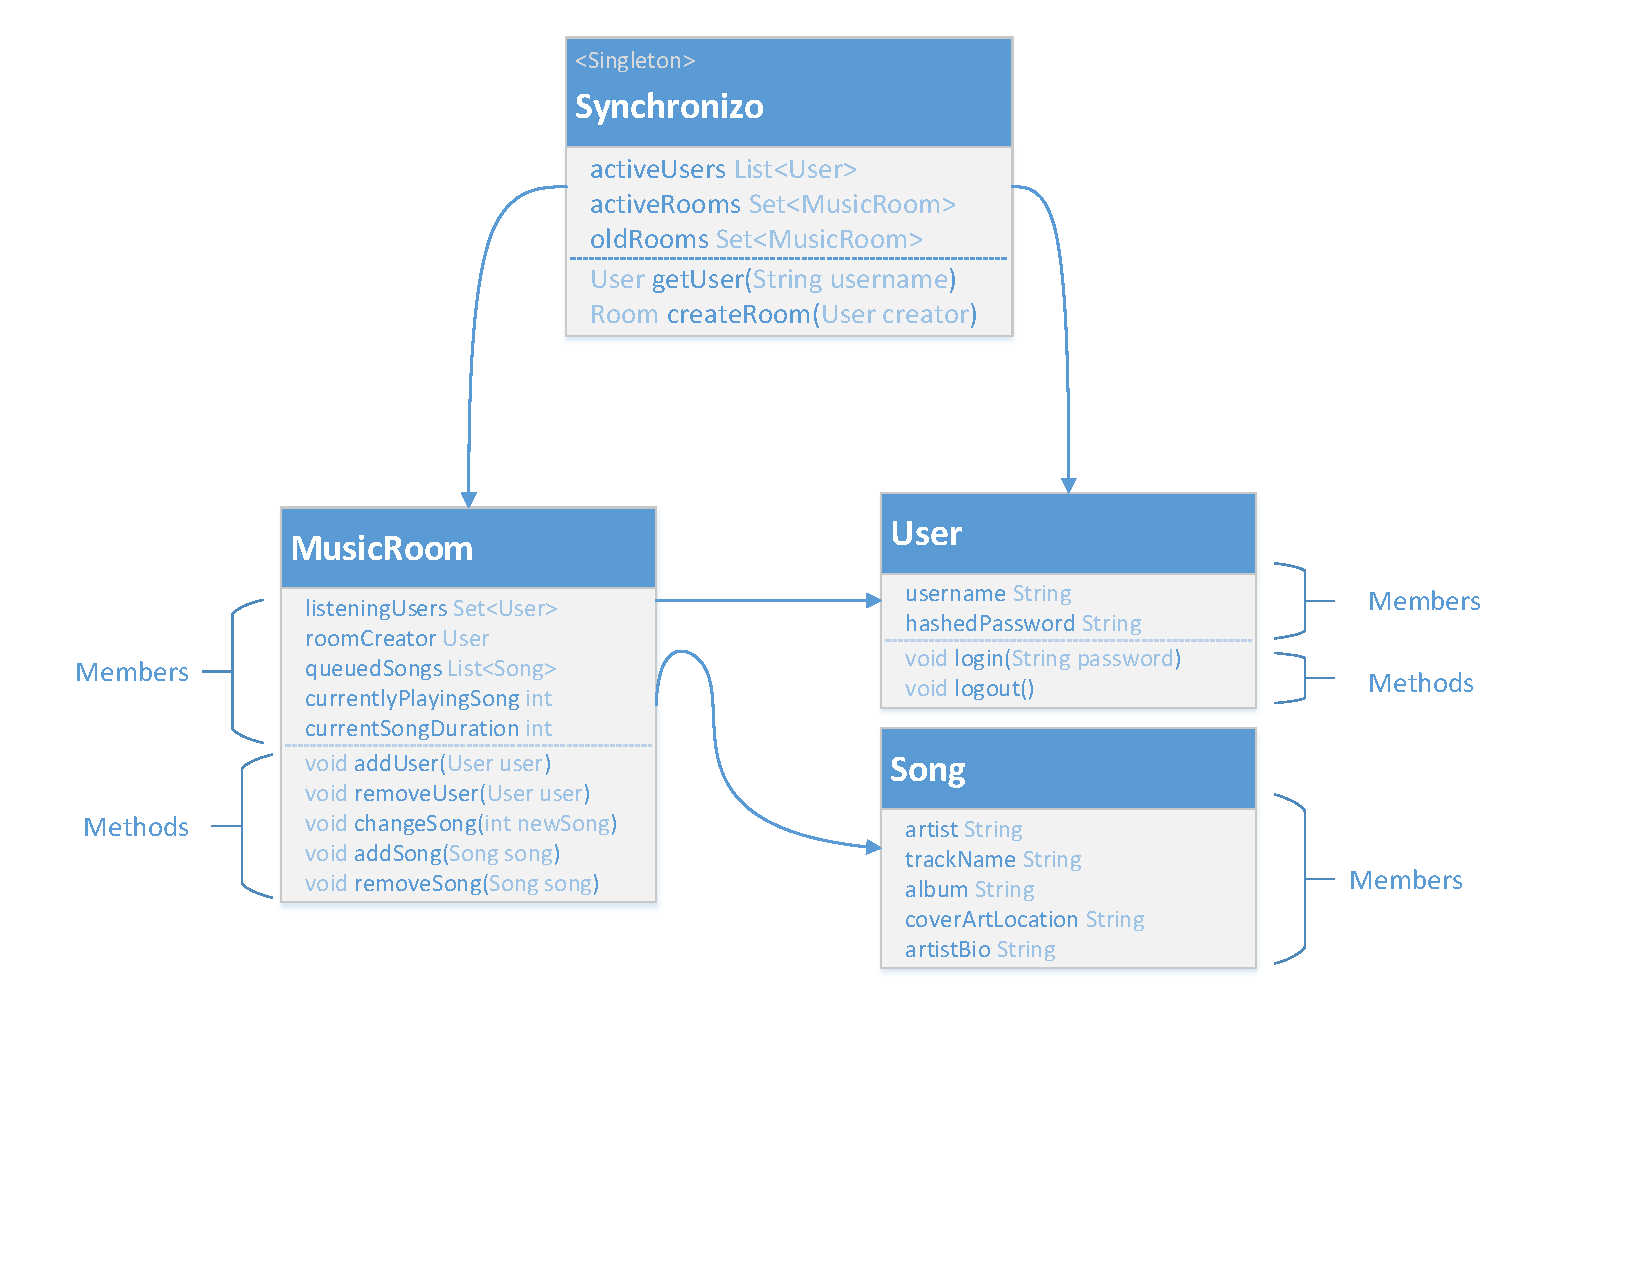
\includegraphics[scale=0.70]{classes.pdf}
\end{center}

These classes encompass the basic ideas for the core functionality of Synchronizo's music listening features. More fields and methods will likely be added to these classes as development actually starts but so far we believe this gives a good overall idea of our class structure.

\begin{description}
    \item [Synchronizo] A singleton (only one instance will be ever created) class that keeps track of the state of the entire web application. This state information includes the currently used music listening rooms, a list of online users and previously used rooms that eventually need to be disbanded.
    
    It also contains methods to access user information from the database, the ability to create new rooms, the ability to delete old rooms, create new users and any methods whose scope is for the entire web app.
    
    \item[MusicRoom] This class represents what would be a room in real life with multiple people listening to the same music, hence the name MusicRoom. The information it needs to contain will include the queued up songs, a list of users who are listening to the music in that room, the song that's currently playing and what duration its at and a history of the chat.
    
    All this information allows us to synchronize the music playing for any new user joining the room. We know the playing song and what point it is at, hence we can make their browser seek to that timestamp.
    
    The methods in this class allow for changing the state of the music room. Much like how a person can enter and leave a room in real life, we have ``addUser'' and ``removeUser''. Then there are methods for adding and removing songs from the queued songs list.
    
    \item[Song] A song represents all the information required about a song, such as who the song is by, what album its from and what the name of the song is and its duration. Depending on if we allow file uploads or use an external API, we will either keep track of where the music file is physically stored or an identifier for the API. 
    
    The artist's Bio field will contain information about the artist pulled from the \textit{last.fm} API in order to add more information to the player. To deduplicate this data, we may consider pulling this information into an \textbf{Artist} class.
    
    Since this class needs to contain information about where to find the actual audio file, there will eventually be methods and fields that accommodate the searching of songs, examining their metadata and duration etc.
    
    \item[Artist] Represents a musical artist, contains information about their name, their biography etc. Used to deduplicate data for the \textbf{Song} class. This information will likely be retrieved using the \textit{last.fm} API.
    
    \item[User] The most important class after a MusicRoom. This represents a user of the Synchronizo application. Initially this will only contain a basic username and password for the user, allowing them to be logged into the service. However, once we start building the social networking aspects of the website this will quickly expand. The user will have a list of users as their friends, a biography for their profile page, a basic representation of their music taste etc.
    
    The methods on this class will deal with a lot of the user to user interaction, such as adding friends, sending messages, blocking users and messaging others. Once administrative abilities have to be built into the website, permissions flagging will be introduced to distinguish ordinary users and administrators.
\end{description}

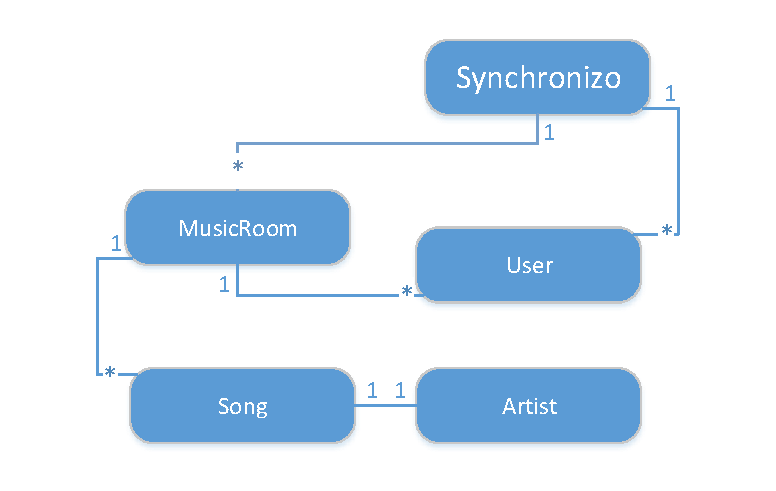
\includegraphics[scale=0.70]{interactions.pdf}

The application can host multiple users and rooms, hence the 1-to-many relation there. Rooms can contain multiple users and songs. A single song will only have one artist associated with it.

\section{Sequence Diagrams}

\subsection{Entering a Room}

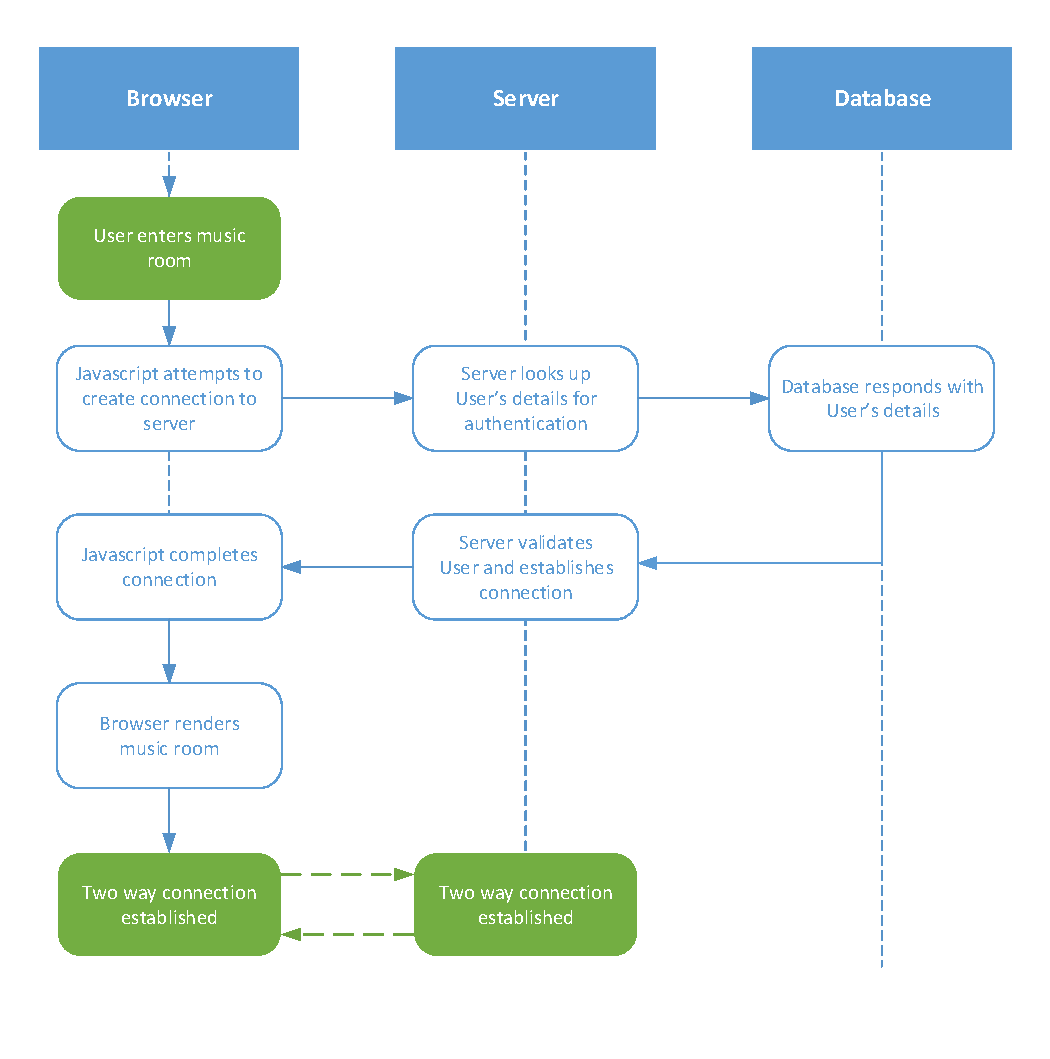
\includegraphics[scale=0.8]{entering_room.pdf}

\subsection{Uploading a Song}

This diagram follows the basic interaction of the system when a user wants to upload a new song. First the browser sends the header of the music file so we can extract the ID3 metadata tags and validate the song, and actively start retrieving information about it, before it has to be fully uploaded. The server then stores information about what the user uploaded persistently in the database and approves the rest of the file upload. Once the file has been uploaded, the server pushes out a notification to all the browsers in the room, so they can then render the information about the new upload locally.

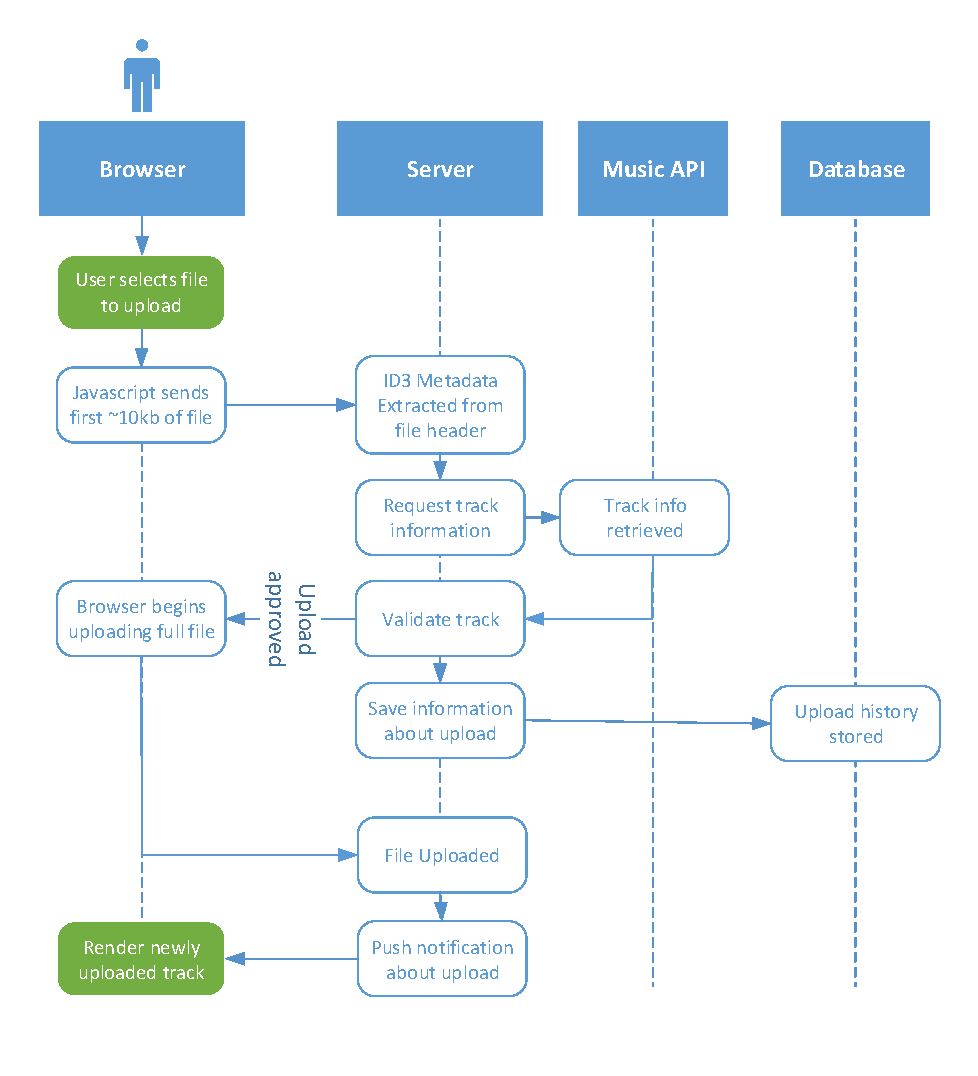
\includegraphics[scale=1]{uploading.pdf}

\pagebreak

\subsection{Seeking a song}

Seeking is clicking the duration bar of a song to skip to a certain time-stamp in it.

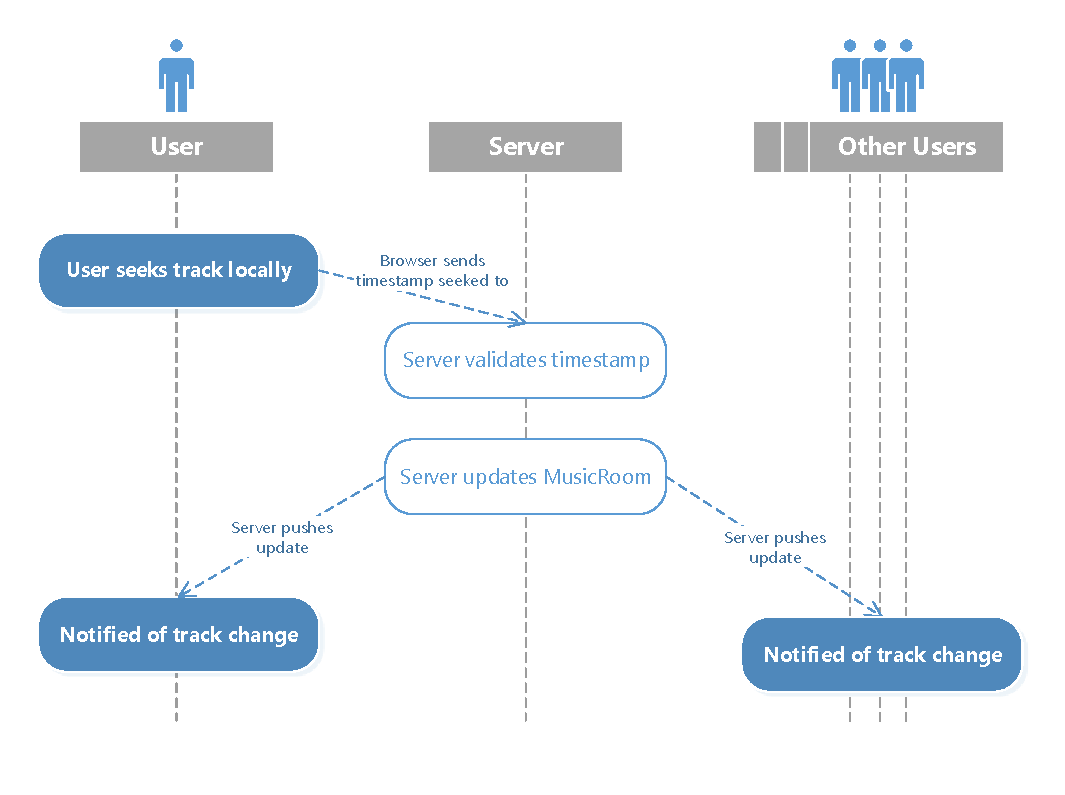
\includegraphics[scale=0.9]{seeking.pdf}

These two interactions pretty much follow all the other interactions in the system. Whenever a user makes a change, the server validates it, processes it and then pushes out updates to other users. The browsers of the other users then render and display these changes locally.

Removing a song will follow a similar course, where a user clicks the remove button, the server validates and checks which track is being removed. It then removes it from the \textbf{MusicRoom} class and proceeds to push out an update to all the clients that the track has been removed. Upon receiving this information, the clients then proceed to remove the displayed track from the HTML of the page, hence completing the sequence.

\Centered{
    \chapter{UI Mockups}
}

\begin{figure}[h]
\centering
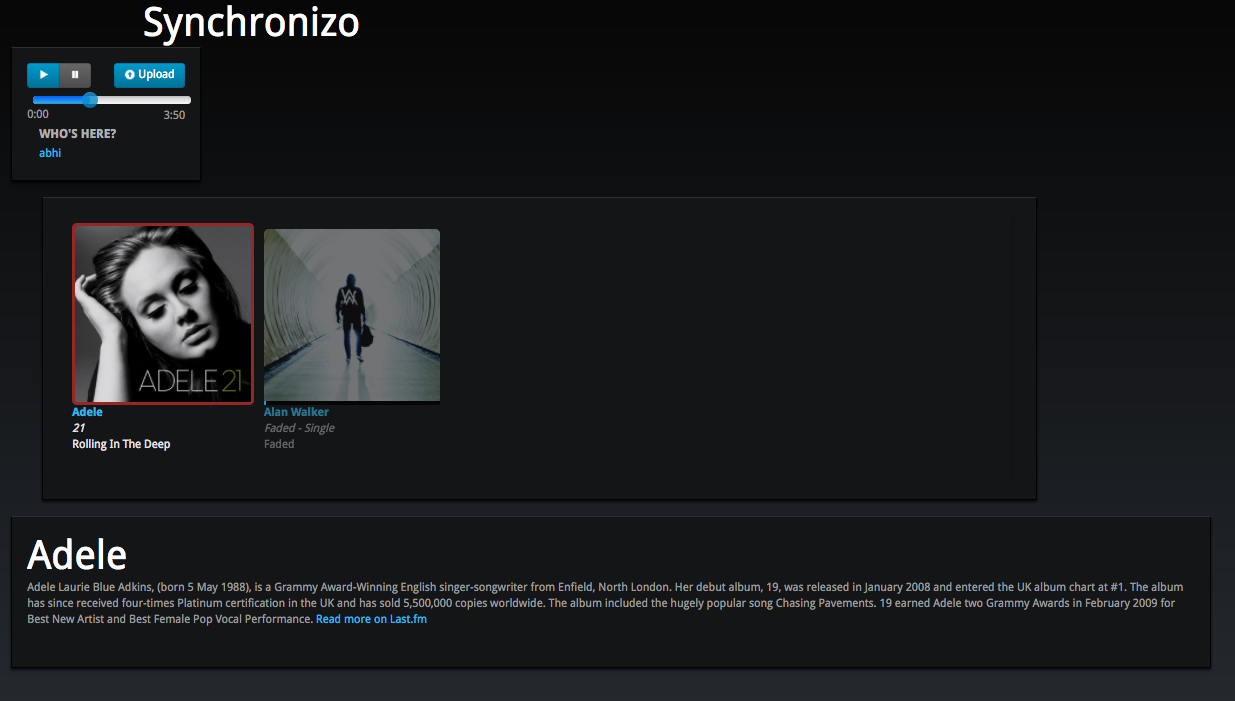
\includegraphics[width=1.0\textwidth]{mockup}
\caption{A basic mockup of the music player}
\end{figure}

\begin{figure}[h]
\centering
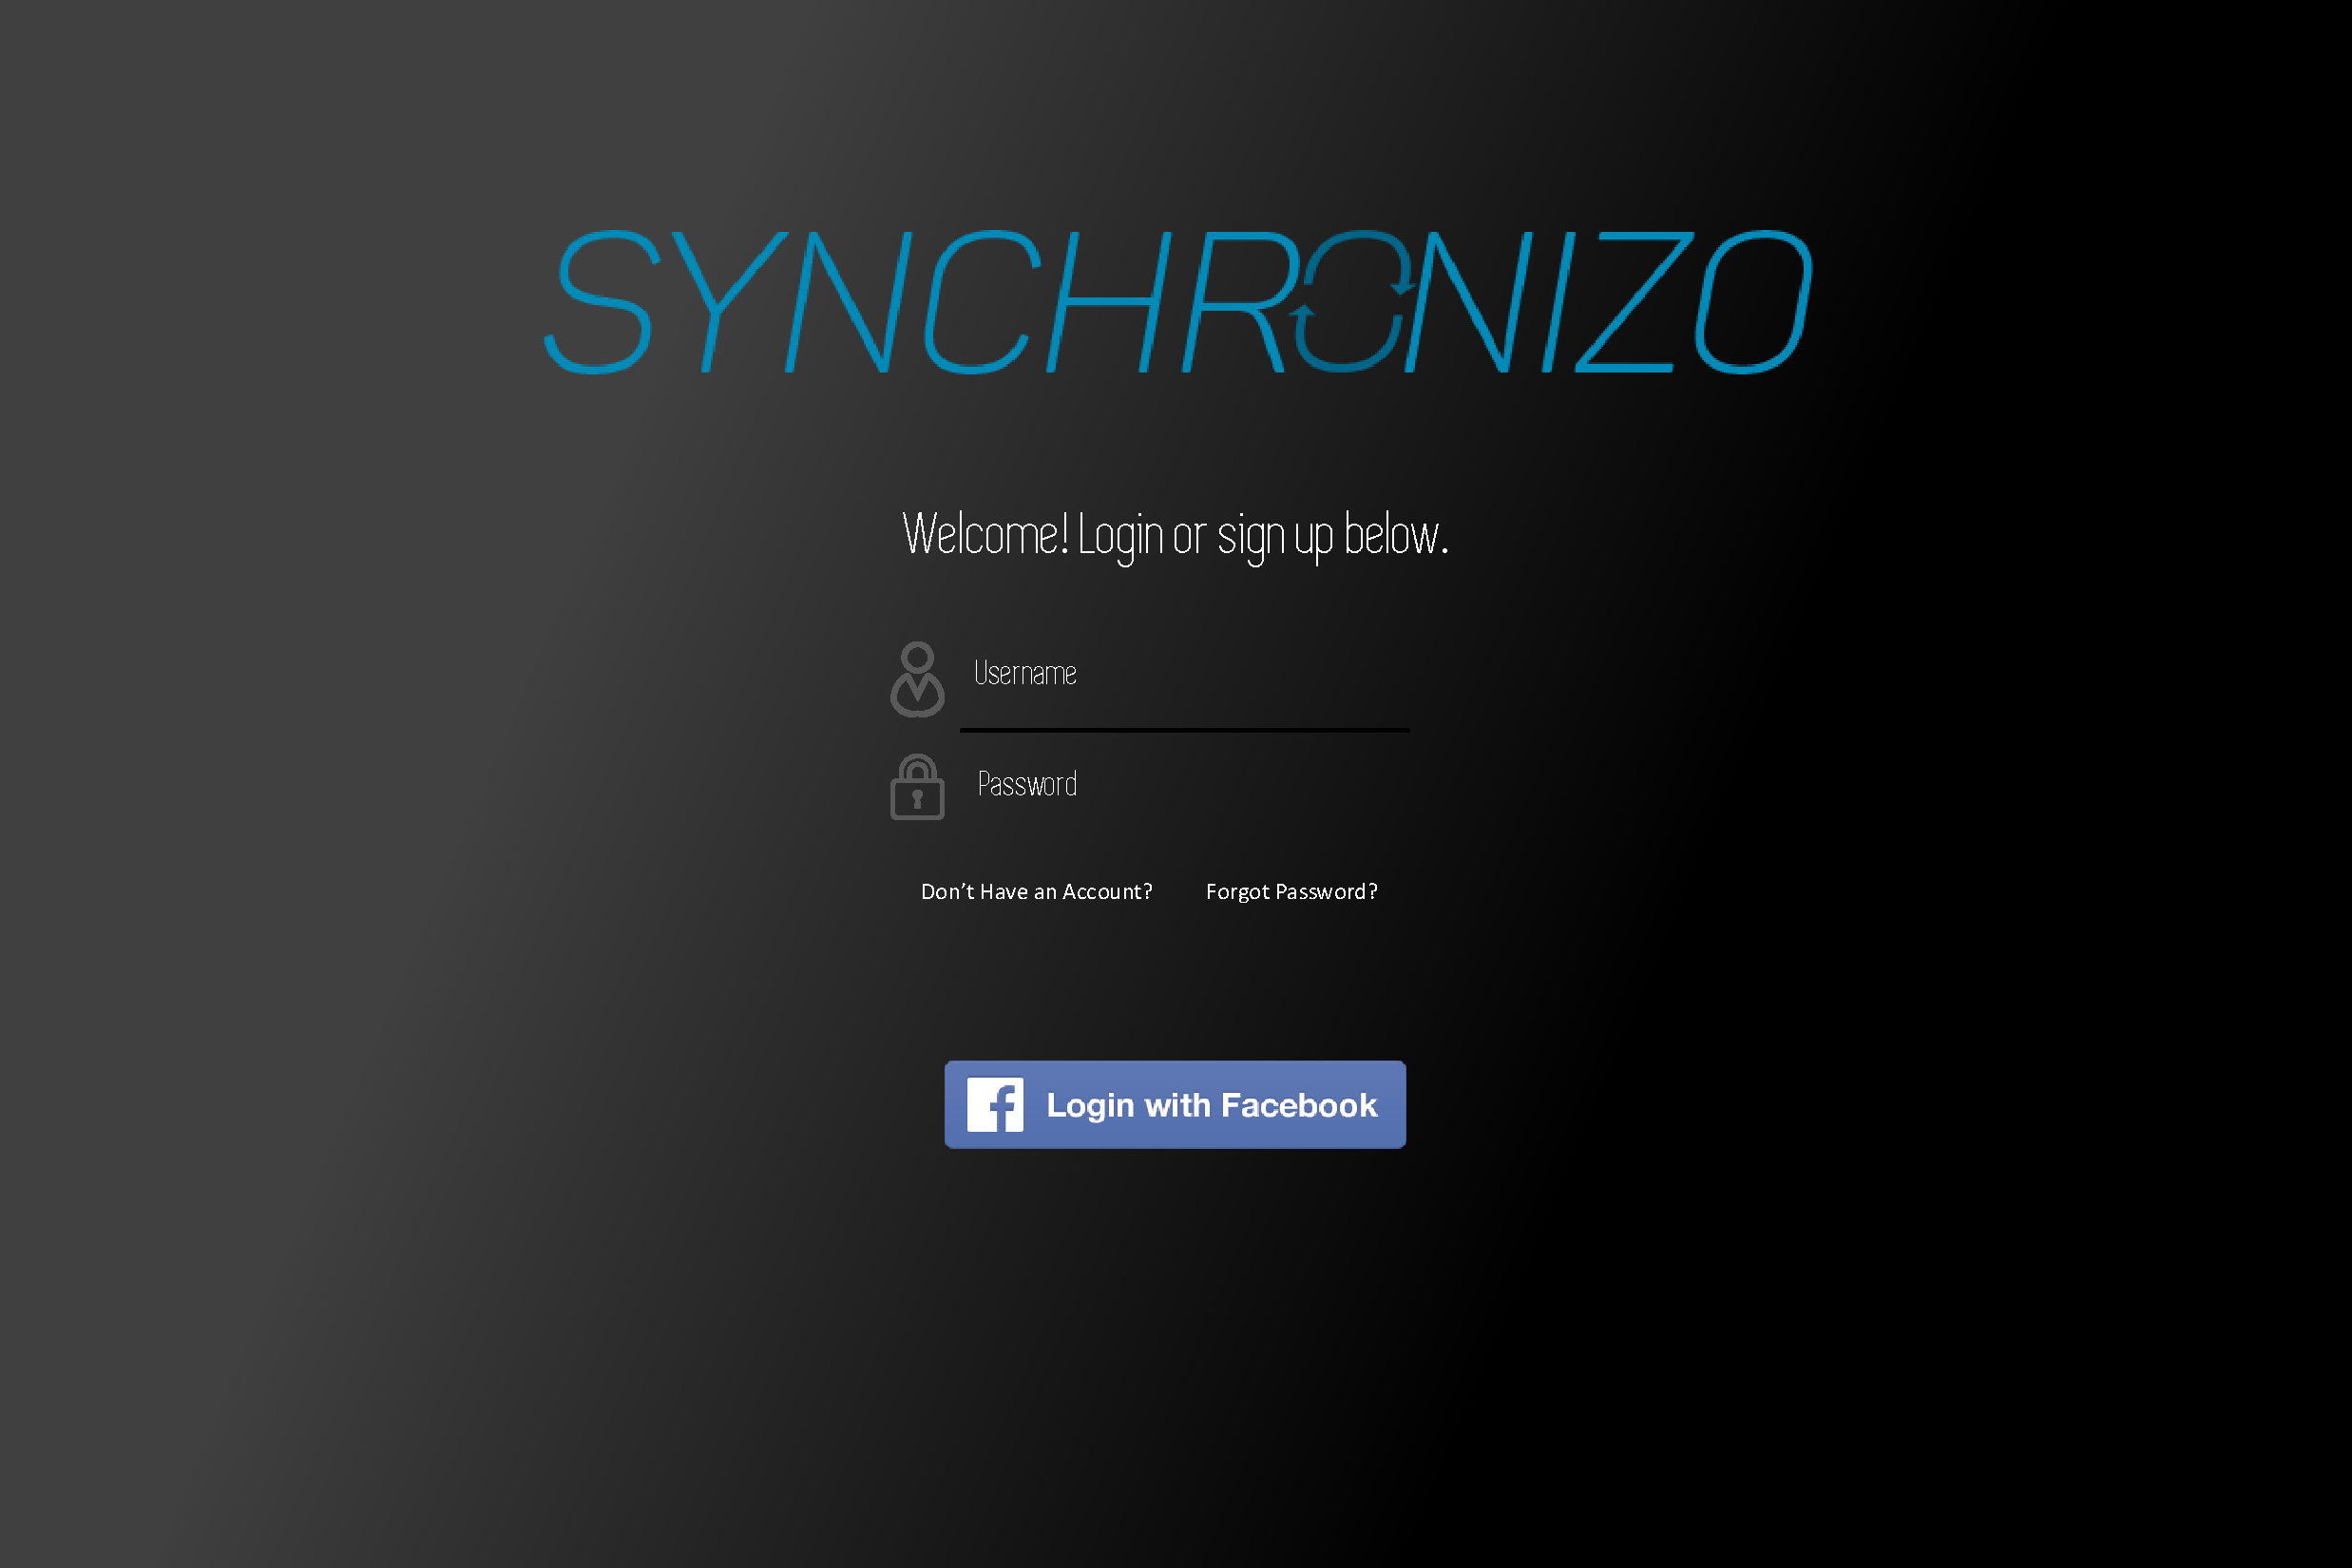
\includegraphics[width=1.0\textwidth]{LoginMockupBlack}
\caption{A mockup of the general layout of the login screen.}
\end{figure}

\end{document}
